\section{Understanding Clustering, Regression and SVMs}

%\subsection{Non-Negative Matrix Factorization}

\subsection{Clustering. Centroids election.}

In this problem, you will see why we define the centroids as the mean of the points in a cluster.

\begin{enumerate}
    \item Let $\{ {\bf a}_1, {\bf a}_2, ... , {\bf a}_n \}$ be a set of $n$ points in a $d$-dimensional space. Show that the sum of the squared distances of the ${\bf a}_i$ to any point ${\bf x}$ equals the sum of the squared distances to the centroid of the ${\bf a}_i$ plus $n$ times the squared distance from ${\bf x}$ to the centroid. That is,
\begin{eqnarray}
\sum_{i = 1}^n \| {\bf a}_i - {\bf x}\|^2 & = & \sum_{i=1}^{ n} \| {\bf a}_i - {\bf c}\|^2 +  n \| {\bf c} - {\bf x}\|^2
\end{eqnarray}
where ${\bf c} = \frac{1}{ n} \sum_{i=1}^n {\bf a}_i$ is the centroid of the set of points.

\item Conclude that the sum of squared distances of the ${\bf a}_i$ to a point ${\bf x}$ is minimized when ${\bf x}$ is the centroid, namely ${\bf x} = \frac{1}{n} \sum_{i} {\bf a}_i$

\end{enumerate}

\subsection{Support Vector Machines}

Use the following dataset in 1-D space which consists of 3 positive data points $\{0, 1, 2\}$ and 3 negative data points $\{ -2, -1, 3\}$.

\begin{figure}[h!]
    \centering
    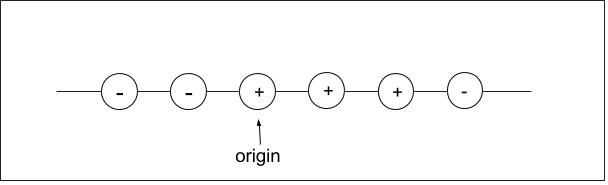
\includegraphics[trim ={0 0 0 0 }, scale=0.4]{figs/problem1.jpg}
    %\caption{Magnitude spectrum (in log scale) of files \texttt{music.wav} and \texttt{speech.wav}}
    \label{face_example}
\end{figure}

\begin{enumerate}
    \item Find a feature map $\varphi \, : \, \mathbb{R}^1 \rightarrow \mathbb{R}^2$ which will map the data in the original 1-D input space $(x)$ to a 2-D feature space $\varphi(x) = (y_1, \, y_2)$ so that the data becomes linearly-separable. Plot the dataset after mapping in 2-D space.
    
    \item Write down the equation for the separator hyperplane $w_0+w_1y_1+w_2y_2 = 0$ given by hard-margin linear SVM in the 2-D feature space. Draw this hyperplane on your plot and mark the corresponding support vector(s).

\end{enumerate}

\subsection{Regularized least squares}

\begin{enumerate}
    \item[] Given $X$, a $m \times n$ matrix, show that the solution to the regularized least-squares problem
\begin{eqnarray}
\min_{\beta} \| {\bf y} - X\beta \|^2 + \lambda \| \beta \|^2
\end{eqnarray}
is
\begin{eqnarray}
\hat{\beta} & = & (X^\top X + \lambda I_n )^{-1} X^\top {\bf y}
\end{eqnarray}
where $I_n$ is the identity matrix of size $n$ and $\lambda>0$.
\end{enumerate}



\iffalse
\newpage
\subsection{Adaboost}

The figure below shows a data set that contains two classes ('+' and 'o'). The instances are labeled A-E.

\begin{center}
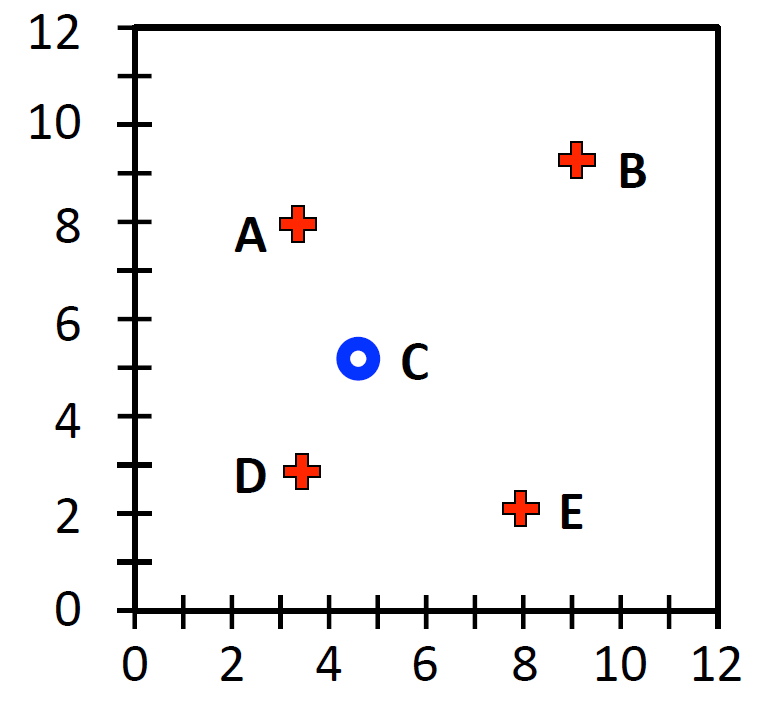
\includegraphics[trim={0cm 0 0 0},clip,scale=0.4]{figs/fig1.png}
\end{center}

If we train Adaboost to solve the classification problem.

\begin{enumerate}
    \item Which instances will have their weights increased at the end of the first boosting iteration? (Explain)
    \item What is the \textbf{minimum} number of iterations that the algorithm could take to achieve zero training error? (Explain)
    \item Is it possible to add another example to the data set to guarantee that boosting achieves zero training error in just two iteration? If so, how? If not, why?
\end{enumerate}

\subsection{Affine Transformation of Random variables}
Let ${\bf X}$ be a $d$-dimensional random vector with mean ${\bf \mu}$ and covariance matrix  $\Sigma$. Let ${\bf Y} = A{\bf X} + {\bf b}$, where $A$ is a $n \times d$ matrix and ${\bf b}$ is a $n$-dimensional vector.

\begin{enumerate}
    \item Show that the mean of ${\bf Y}$ is $A {\bf \mu } + {\bf b}$
    \item Show that the covariance matrix ${\bf Y}$ is $A \Sigma A^\top$
\end{enumerate}

\subsection{Difference between Correlation and Independence}

Consider the discrete random variable $X$ described as follows
$$ \mathbb{P}(X = i ) = \left\{ \begin{array}{ll} 1/3 & \text{ if } i = -1\\
1/3 & \text{ if } i = 0\\
1/3 & \text{ if } i = 1\end{array}\right.$$
We also define the random variable $Y = 1 - X^2$.

\begin{enumerate}
    \item Compute the values of $\mathbb{E}(X)$ and $\mathbb{E}(Y)$.
    \item Compute $\mathbb{E}(XY)$ and $Cov(X,Y)$. Are $X$ and $Y$ uncorrelated?
    \item Are $X$ and $Y$ independent? i.e., $\mathbb{P}(X = i\, , \, Y=j) = \mathbb{P}(X = i) \mathbb{P}(Y =j)$?
\end{enumerate}
\fi




